\section{Variables} \label{vr}
\subsection{Primer Objetivo} \label{vr:1o}
Por cada movimiento se debe enumerar las articulaciones que ayudan a un usuario a moverse, de igual manera, enumerar los pasos que se debe seguir para ejecutar la acci\'on -i.e. Repetici\'on del movimiento-.
\subsubsection{Variables dependientes} \label{vr:1o:dep}
\begin{enumerate}
	\item[A.] \textbf{Articulaciones del movimiento:}  Vector de enteros la cual se almacena el valor del enumerador, JointType, del SDK de  \citeA{microsoftJointKinect}.
	\item[B.] \textbf{N\'umeros de pasos}: Valor positivo, mayor a 1.
\end{enumerate}
	\begin{figure}[H]
	\caption{Variables dependientes del primer objetivo}
	\label{fig:vardep1}
	\centering
	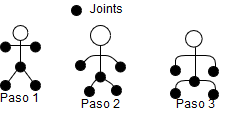
\includegraphics[width=300px,height=100px]{graphics/var-1obj.png} \\
	\textbf{Fuente:}Elaboraci\'on propia 
\end{figure}
\medbreak
\begin{table}[H]
\begin{center}
\caption{Definiciones de variables dependientes del primer objetivo}
\label{tab:def1o}
\begin{tabular}{|l|l|l|}
\hline
Enumeraci\'on & Definici\'on Operacional & Definici\'on conceptual \\
\hline
\ref{vr:1o:dep}.A & \begin{tabular}[c]{@{}l@{}}Son aquellas articulaciones\\ que interviene para realizar\\ el movimiento -i.e. Arcos\\ de movibilidad-.\end{tabular} & \begin{tabular}[c]{@{}l@{}}Conjunto de \'indices enteros \\ que representa las articulaciones\\ (ver figura \ref{fig:jointsKinect}) y arcos de\\ movibilidad (ver figuras \ref{fig:ArcosdeMovilidad} y \ref{fig:ArcosdeMovilidad2})\\ del seguimiento del esqueleto \end{tabular}  \\
\hline
\ref{vr:1o:dep}.B & \begin{tabular}[c]{@{}l@{}}Cantidad de pasos de an\'alisis\\ que tiene el movimiento\end{tabular} & \begin{tabular}[c]{@{}l@{}}De acuerdo a las variables del \\  movimiento (ver secci\'on \ref{mt:mf:var}), \\ los pasos define la coordinaci\'on \\ del movimiento\end{tabular}\\
\hline
\end{tabular}
\end{center}
\textbf{Fuente:} Elaborado por el autor de tesis
\end{table}
\subsection{Tercer Objetivo} \label{vr:3o}
Por cada movimiento es necesario indicar la articulaci\'on de an\'alisis -i.e. Punto central de estudio-,  la cual a partir de ella se calcula la distancia de profundidad m\'inima y m\'axima, con la finalidad de que el seguimiento de esqueleto tenga un menor error posible, sin embargo esta funcionalidad depende de la altura de usuario y el Kinect. 
\subsubsection{Variables dependientes} \label{vr:3o:dep}
\begin{enumerate}
	\item[A.] \textbf{Articulaci\'on de an\'alisis}: Valor entero que pertenece al  enumerador, JointType, del SDK de \citeA{microsoftJointKinect}. 
	\item[B.] \textbf{Altura del usuario}: Valor decimal positivo -i.e. Medida en metros- que se determina a partir de los componentes de altura de las articulaciones de la cabeza y p\'ies del usuario.	 
	\item[C.] \textbf{Altura del kinect respecto al suelo}: Valor decimal positivo -i.e. Medida en metros- que permanece constante por movimiento. 
\end{enumerate}
\medbreak
\begin{figure}[H]
	\caption{Variables dependientes del tercer objetivo}
	\label{fig:vardep3}
	\centering
	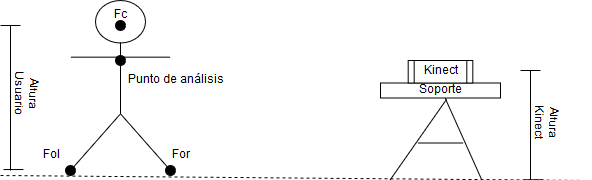
\includegraphics[width=300px,height=100px]{graphics/var-3obj.png} \\
	\textbf{Fuente:}Elaboraci\'on propia 
\end{figure}
\medbreak
\begin{table}[H]
\begin{center}
\caption{Definiciones de variables dependientes del Tercer objetivo}
\label{tab:def3o}
\begin{tabular}{|l|l|l|}
\hline
Enumeraci\'on & Definici\'on Operacional & Definici\'on conceptual \\
\hline
\ref{vr:3o:dep}.A & \begin{tabular}[c]{@{}l@{}}Articulaci\'on que ayuda\\ a determinar las distancias\\ m\'aximas y m\'inimas\\ de profundidad\end{tabular} & \begin{tabular}[c]{@{}l@{}}Articulaci\'on del seguimiento de \\ de esqueleto (ver figura \ref{fig:jointsKinect}), que\\ permite realizar el an\'alisis del movimiento,\\ tal como se muestra en los trabajos \\ relacionados (Ver secci\'on \ref{tr}) \end{tabular}  \\
\hline
\ref{vr:3o:dep}.B & \begin{tabular}[c]{@{}l@{}}Variable de referencia para \\ ubicar al usuario en la profundidad \\ adecuada del seguimiento \\ del esqueleto\end{tabular} & \begin{tabular}[c]{@{}l@{}}La altura es una variable que puede \\ afectar los movimientos cinem\'aticos \\ (ver secci\'on \ref{mt:cam:kin}.\ref{mt:cam:kin:vgb}), \\ dado que afecta las dimensiones \\ del seguimiento de esqueleto\end{tabular}\\
\hline
\ref{vr:3o:dep}.C & \begin{tabular}[c]{@{}l@{}}Variable que permanece constante\\ por movimiento, adem\'as de ser \\ el punto central de  \\ captura de datos del Kinect\end{tabular} & \begin{tabular}[c]{@{}l@{}}La transmici\'on de datos del Kinect \\ (ver figura \ref{fig:interaccionKinect}) tendr\'a un menor error, \\  si se posiciona a una altura, \\  donde el sensor tenga un \\  mayor campo de visi\'on (ver figura \ref{fig:RGBESP} ) \end{tabular}\\
\hline
\end{tabular}
\end{center}
\textbf{Fuente:} Elaborado por el autor de tesis
\end{table}
\subsubsection{Variables independientes} \label{vr:3o:indep}
\begin{enumerate}
	\item[A.] \textbf{Distancia m\'inima de profundidad del movimiento}: Valor decimal positivo -i.e. Medida en metros- que determina la distancia m\'inima adecuada para ejecutar el seguimiento de esqueleto.
	\item[B.] \textbf{Distancia m\'axima de profundidad del movimiento}: Valor decimal positivo -i.e. Medida en metros- que determina la distancia m\'axima adecuada para ejecutar el seguimiento de esqueleto.
\end{enumerate}
\medbreak
\begin{figure}[H]
	\caption{Variables independientes del tercer objetivo}
	\label{fig:varindep3}
	\centering
	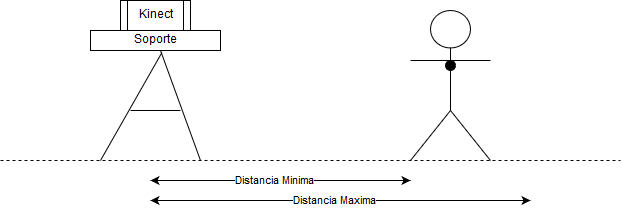
\includegraphics[width=300px,height=100px]{graphics/var-3obj-ind.png} \\
	\textbf{Fuente:}Elaboraci\'on propia 
\end{figure}
\medbreak
\begin{table}[H]
\begin{center}
\caption{Definiciones de variables independientes del Tercer objetivo}
\label{tab:def3o2}
\begin{tabular}{|l|l|l|}
\hline
Enumeraci\'on & Definici\'on Operacional & Definici\'on conceptual \\
\hline
\ref{vr:3o:indep}.A & \begin{tabular}[c]{@{}l@{}}Distancia m\'inima la\\ cual detecta todo el\\ esqueleto del usuario\\ -i.e. desde la cabeza \\ hasta los p\'ies-.\end{tabular} & \multirow{2}{*}{\begin{tabular}[c]{@{}l@{}} El seguimiento de esqueleto\\ depende del alcance del sensor \\ de profundidad y el campo \\ de visi\'on (ver figura \ref{fig:RGBESP}). \end{tabular}} \\
\cline{1-2}
\ref{vr:3o:indep}.B & \begin{tabular}[c]{@{}l@{}}Distancia m\'axima la\\ cual deja de detectar\\ todo el esqueleto del \\  usuario. \end{tabular} & \\
\hline
\end{tabular}
\end{center}
\textbf{Fuente:} Elaborado por el autor de tesis
\end{table}
\subsection{Cuarto Objetivo} \label{vr:4o}
Durante un movimiento, una articulaci\'on se desplaza durante un per\'iodo de tiempo.
\subsubsection{Variables dependientes} \label{vr:4o:dep}
\begin{enumerate}
	\item[A.] \textbf{Tiempo de captura de datos}: Valor decimal positivo -i.e. Medida en segundos-, la cual mide el tiempo del movimiento de una articulaci\'on.
\end{enumerate}
\medbreak
\begin{figure}[H]
	\caption{Variables dependientes del cuarto objetivo}
	\label{fig:vardep4}
	\centering
	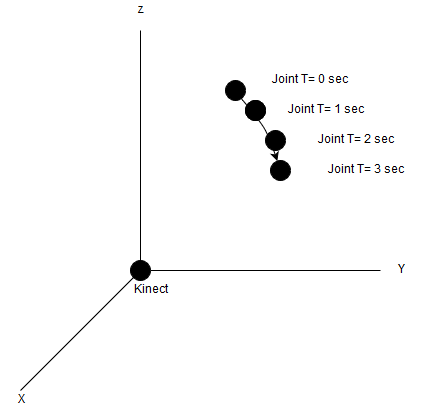
\includegraphics[width=180px,height=100px]{graphics/var-4obj.png} \\
	\textbf{Fuente:}Elaboraci\'on propia 
\end{figure}
\begin{table}[H]
\begin{center}
\caption{Definiciones de variables dependientes del cuarto objetivo}
\label{tab:def4o}
\begin{tabular}{|l|l|l|}
\hline
Enumeraci\'on & Definici\'on Operacional & Definici\'on conceptual \\
\hline
\ref{vr:4o:dep}.A & \begin{tabular}[c]{@{}l@{}}Unidad de tiempo \\  con respecto al \\ movimiento de an\'alisis\end{tabular} & \begin{tabular}[c]{@{}l@{}}De acuerdo a la resoluci\'on de 3D  \\ y del color (ver tabla \ref{tab:RGBD}), \\ el Kinect percibe un total \\ 30 frames por segundos, \\ lo cual puede llegar a  \\  capturar los datos cada \\  0.033 segundos. \end{tabular}  \\
\hline
\end{tabular}
\end{center}
\textbf{Fuente:} Elaborado por el autor de tesis
\end{table}
\subsubsection{Variables independientes} \label{vr:4o:indep}
\begin{enumerate}
	\item[A.] \textbf{Desplazamiento de la articulaci\'on}: Valor decimal positivo -i.e. Medida en metros- que determina la distancia de una articulac\'on y un punto de origen -i.e. Kinect-:
\end{enumerate}
\medbreak
\begin{figure}[H]
	\caption{Variables independientes del cuarto objetivo}
	\label{fig:varIdep4}
	\centering
	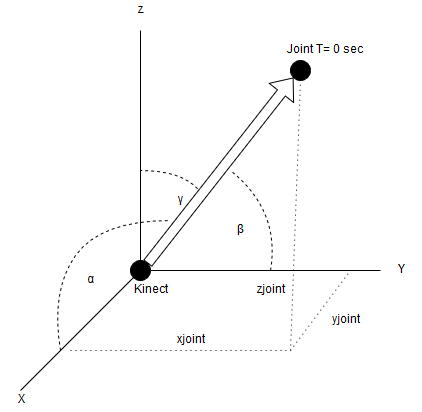
\includegraphics[width=230px,height=150px]{graphics/var-4obj-ind.png} \\
	\textbf{Fuente:}Elaboraci\'on propia 
\end{figure}
\begin{table}[H]
\begin{center}
\caption{Definiciones de variables independientes del cuarto objetivo}
\label{tab:def4oI}
\begin{tabular}{|l|l|l|}
\hline
Enumeraci\'on & Definici\'on Operacional & Definici\'on conceptual \\
\hline
\ref{vr:4o:indep}.A & \begin{tabular}[c]{@{}l@{}}Valor que muestra el desplazamiento \\ de la articulaci\'on de an\'alisis \\ -i.e. C\'omo se esta \\ moviendo el cuerpo-. \end{tabular} & \begin{tabular}[c]{@{}l@{}}De acuerdo a las variables \\ de un movimiento (ver secci\'on \ref{mt:mf:var}) \\ y movimientos cin\'ematicos  \\ (ver secci\'on \ref{mt:cam:kin}.\ref{mt:cam:kin:vgb}),  \\ el desplazamiento permite calcular \\ la velocidad y aceleraci\'on \\ de un movimiento \\ a partir de la posici\'on  \\ de una articulaci\'on \\ (ver figura  \ref{fig:CoordenadaJoint})\\ con respecto al \\ tiempo de movimiento \end{tabular}  \\
\hline
\end{tabular}
\end{center}
\textbf{Fuente:} Elaborado por el autor de tesis
\end{table}
\subsection{Quinto Objetivo} \label{vr:5o}
Por cada movimiento se le debe asignar una etiqueta a cada paso y su rango m\'aximo de identificaci\'on, para encontrar el valor del factor de movimiento.
\subsubsection{Variables dependientes} \label{vr:5o:dep}
\begin{enumerate}
	\item[A.] \textbf{Etiquetas}: Vector de valores decimales entre 0 a 1.  
	\item[B.] \textbf{Rango m\'aximo de identificaci\'on}: Vector que almacena un vector n\'umerico.
\end{enumerate}	 
\medbreak
\begin{figure}[H]
	\caption{Variables dependientes del quinto objetivo}
	\label{fig:vardep5}
	\centering
	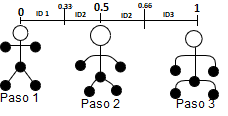
\includegraphics[width=180px,height=100px]{graphics/var-5obj.png} \\
	\textbf{Fuente:}Elaboraci\'on propia 
\end{figure}
\medbreak
\begin{table}[H]
\begin{center}
\caption{Definiciones de variables dependientes del quinto objetivo}
\label{tab:def5oI}
\begin{tabular}{|l|l|l|}
\hline
Enumeraci\'on & Definici\'on Operacional & Definici\'on conceptual \\
\hline
\ref{vr:5o:dep}.A & \begin{tabular}[c]{@{}l@{}}Valor que identifica \\ el paso de un movimiento. \end{tabular} & \begin{tabular}[c]{@{}l@{}}De acuerdo a las variables \\ de un movimiento (ver secci\'on \ref{mt:mf:var}) \\  los coordinaci\'on hace referencia \\ a las etiquetas del movimiento \\ (ver figura \ref{fig:modeloContinuo}). \end{tabular}  \\ \hline
\ref{vr:5o:dep}.B & \begin{tabular}[c]{@{}l@{}}Detalla el paso \\ que realiza   \\ el  factor del  \\ movimiento. \end{tabular} & \begin{tabular}[c]{@{}l@{}}De acuerdo a las variables \\ de un movimiento (ver secci\'on \ref{mt:mf:var}) \\  el rango equivale \\ a la precisi\'on del movimiento \\ (ver figura \ref{fig:modeloContinuo}). \end{tabular}  \\
\hline
\end{tabular}
\end{center}
\textbf{Fuente:} Elaborado por el autor de tesis
\end{table}
\subsubsection{Variables independientes} \label{vr:5o:indep}
\begin{enumerate}
	\item[A.] \textbf{Factor de movimiento}: valor  decimal entre 0 a 1, la cual representa la probabilidad del seguimiento de un movimiento.
\end{enumerate}	
\medbreak
\begin{figure}[H]
	\caption{Variables independientes del quinto objetivo}
	\label{fig:varIdep5}
	\centering
	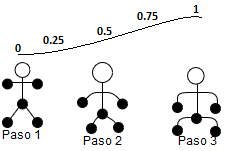
\includegraphics[width=180px,height=100px]{graphics/var-5obj-ind.png} \\
	\textbf{Fuente:}Elaboraci\'on propia 
\end{figure}
\medbreak
\begin{table}[H]
\begin{center}
\caption{Definiciones de variables independientes del quinto objetivo}
\label{tab:def5oI}
\begin{tabular}{|l|l|l|}
\hline
Enumeraci\'on & Definici\'on Operacional & Definici\'on conceptual \\
\hline
\ref{vr:5o:indep}.A & \begin{tabular}[c]{@{}l@{}}Valor que identifica \\ el seguimiento del movimiento \\ en tiempo real \end{tabular} & \begin{tabular}[c]{@{}l@{}}Variable que se calcula  \\ a partir del modelo Random  \\ Forest Regression (ver \\ seccio\'n \ref{mt:cam:kin}.\ref{mt:cam:kin:vgb}) \end{tabular}  \\
\hline
\end{tabular}
\end{center}
\textbf{Fuente:} Elaborado por el autor de tesis
\end{table}
\subsection{S\'eptimo Objetivo} \label{vr:7o}
Una rutina es configurada a partir de un n\'umero de series de tiempo de trabajo y descanso, en donde el usuario realiza las m\'aximas repeticiones posibles del movimiento  durante el tiempo de trabajo, tomando en cuenta que la repetici\'on debe pasar por todos los pasos definidos (ver variable \ref{vr:1o:dep}.B).
\subsubsection{Variables dependientes} \label{vr:7o:dep}
\begin{enumerate}
	\item[A.] \textbf{Tiempo de descanso}: Valor entero positivo -i.e. Medida en segundos-, la cual debe ser menor o igual al tiempo de trabajo.
	\item[B.] \textbf{Tiempo de Trabajo}: Valor entero positivo -i.e. Medida en segundos-.
	\item[C.] \textbf{Cantidad de series}: Valor entero positivo mayor a cero.
\end{enumerate}	
\begin{figure}[H]
	\caption{Variables dependientes del s\'eptimo  objetivo}
	\label{fig:vardep7}
	\centering
	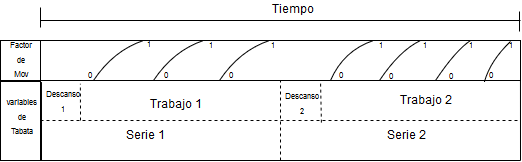
\includegraphics[width=300px,height=100px]{graphics/var-7obj.png} \\
	\textbf{Fuente:}Elaboraci\'on propia 
\end{figure}
\medbreak
\begin{table}[H]
\begin{center}
\caption{Definiciones de variables dependientes del s\'eptimo objetivo}
\label{tab:def7}
\begin{tabular}{|l|l|l|}
\hline
Enumeraci\'on & Definici\'on Operacional & Definici\'on conceptual \\
\hline
\ref{vr:7o:dep}.A & \begin{tabular}[c]{@{}l@{}}Valor que controla el \\ tiempo que debe descansar \\ un usuario durante \\ su rutina -i.e. No \\ se cuenta repeticiones-. \end{tabular} & \multirow{3}{*}{\begin{tabular}[c]{@{}l@{}}Estas variables son \\  definidas a partir de \\ la rutina, Tabata, debido \\ que es un entrenamiento controlado \\  de alta intensidad, \\ cuyo resultado es \\ una mayor metabolizaci\'on \\ del cuerpo  (ver secci\'on \ref{mt:mf:rut}.\ref{mt:mf:rut:hiit})\end{tabular}} \\  
\cline{1-2}
\ref{vr:7o:dep}.B & \begin{tabular}[c]{@{}l@{}}Valor que controla el \\ tiempo que debe trabajar \\ un usuario durante \\ su rutina -i.e. Realizar \\ las m\'aximas repeticiones-. \end{tabular} & \\  
\cline{1-2}
\ref{vr:7o:dep}.C & \begin{tabular}[c]{@{}l@{}}Valor que controla la \\ cantidad de tiempos de \\ trabajos y descanso \\ en una rutina. \end{tabular} &  \\  
\hline
\end{tabular}
\end{center}
\textbf{Fuente:} Elaborado por el autor de tesis
\end{table}
\subsubsection{Variables independientes} \label{vr:7oi:indep}
\begin{enumerate}
	\item[A.] \textbf{Detalle del paso}: Es un vector de valores n\'umericos, en donde contiene el factor de movimiento, n\'umero de paso y la matriz de articulaciones -i.e. Esqueleto-. 
	\item[B.] \textbf{Repetici\'on}:  Es un vector de detalle de todos los pasos definido por el movimiento.
\end{enumerate}	
\medbreak
\begin{table}[H]
\begin{center}
\caption{Definiciones de variables independientes del s\'eptimo objetivo}
\label{tab:defoi7}
\begin{tabular}{|l|l|l|}
\hline
Enumeraci\'on & Definici\'on Operacional & Definici\'on conceptual \\
\hline
\ref{vr:7oi:indep}.A & \begin{tabular}[c]{@{}l@{}}Variable que almacena informaci\'on \\ del esqueleto humano \\ -i.e. posici\'on de cada \\ articulaci\'on-, con respecto \\  a cada paso del movimiento  \end{tabular} &  \begin{tabular}[c]{@{}l@{}}El seguimiento de esqueleto \\ puede ser dibujado en \\ una imagen 2D (ver figura \ref{fig:skeletanTracking}), \\  la cual proporciona \\ la posici\'on de cada articulaci\'on, \\ con el fin objetivo  de \\ calcular la agilidad \\ del movimiento (ver secci\'on \ref{mt:mf:var})\end{tabular}\\
\hline
\ref{vr:7oi:indep}.B & \begin{tabular}[c]{@{}l@{}}Variable que almacena informaci\'on \\ de todos los pasos \\ en orden cronol\'ogico  \\ -e.g. la informaci\'on del paso 1 \\ es guardada antes del paso 2-. \\ Se debe tomar en cuenta \\ que la repetici\'on ser\'a \\ contable, si tiene todos \' los pasos  \end{tabular} & \begin{tabular}[c]{@{}l@{}}Variable que permite \\ contabilizar la actividad \\ f\'isica de una persona  \\  (ver secci\'on \ref{mt:af:var})\end{tabular}\\  
\hline
\end{tabular}
\end{center}
\textbf{Fuente:} Elaborado por el autor de tesis
\end{table}